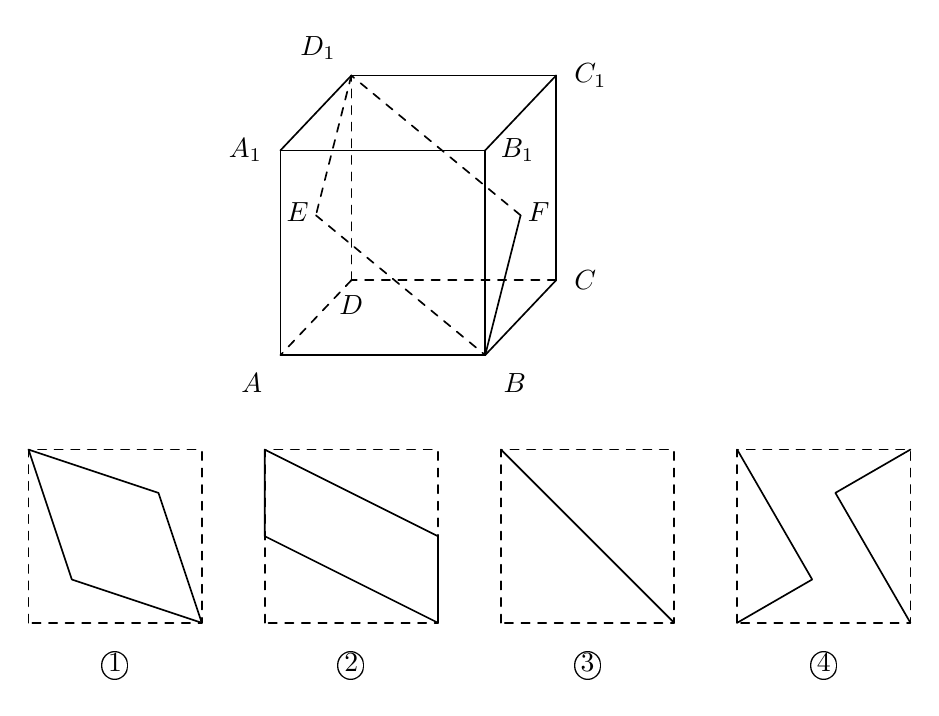
\begin{tikzpicture}[line width=0.6pt, line join=round, line cap=round, font=\normalsize]
  % ---- top cube ----
  \coordinate (A) at (0,0);
  \coordinate (B) at (2.6,0);
  \coordinate (C) at (3.5,0.95);
  \coordinate (D) at (0.9,0.95);
  \coordinate (A1) at (0,2.6);
  \coordinate (B1) at (2.6,2.6);
  \coordinate (C1) at (3.5,3.55);
  \coordinate (D1) at (0.9,3.55);
  \coordinate (E) at (0.4500000000,1.7750000000);
  \coordinate (F) at (3.0500000000,1.7750000000);
  % bottom face
  \draw (A) -- (B);
  \draw (B) -- (C);
  \draw[dashed] (C) -- (D);
  \draw[dashed] (D) -- (A);
  % top face
  \draw (A1) -- (B1);
  \draw (B1) -- (C1);
  \draw (C1) -- (D1);
  \draw (D1) -- (A1);
  % verticals
  \draw (A) -- (A1);
  \draw (B) -- (B1);
  \draw (C) -- (C1);
  \draw[dashed] (D) -- (D1);
  % quadrilateral B-F-D1-E
  \draw[dashed] (D1) -- (E);
  \draw[dashed] (E) -- (B);
  \draw (B) -- (F);
  \draw[dashed] (F) -- (D1);
  % cube labels with clearance
  \node[below left=3pt] at (A) {$A$};
  \node[below right=3pt] at (B) {$B$};
  \node[right=3pt] at (C) {$C$};
  \node[below=2pt] at (D) {$D$};
  \node[left=3pt] at (A1) {$A_{1}$};
  \node[right=2pt] at (B1) {$B_{1}$};
  \node[right=3pt] at (C1) {$C_{1}$};
  \node[above left=2pt] at (D1) {$D_{1}$};
  \node[left=4pt,xshift=5pt,yshift=1pt] at (E) {$E$};
  \node[right=4pt,xshift=-5pt,yshift=1pt] at (F) {$F$};
  % ---- four projection options below ----
  \begin{scope}[shift={(-3.2,-3.4)}]
    \draw[dashed] (0,0) rectangle (2.2,2.2);
    \draw (0,2.2) -- (1.65,1.65) -- (2.2,0) -- (.55,.55) -- cycle;
    \node[below=6pt] at (1.1,-0.05) {\textcircled{1}};
  \end{scope}
  \begin{scope}[shift={(-0.2,-3.4)}]
    \draw[dashed] (0,0) rectangle (2.2,2.2);
    \draw (0,2.2)--(2.2,1.1)--(2.2,0)--(0,1.1)--cycle;
    \node[below=6pt] at (1.1,-0.05) {\textcircled{2}};
  \end{scope}
  \begin{scope}[shift={(2.8,-3.4)}]
    \draw[dashed] (0,0) rectangle (2.2,2.2);
    \draw (0,2.2) -- (2.2,0);
    \node[below=6pt] at (1.1,-0.05) {\textcircled{3}};
  \end{scope}
  \begin{scope}[shift={(5.8,-3.4)}]
    \draw[dashed] (0,0) rectangle (2.2,2.2);
    \draw (0,2.2) -- (0.9526279442,.55) -- (0,0);
    \draw (2.2,2.2) -- (1.2473720558,1.65) -- (2.2,0);
    \node[below=6pt] at (1.1,-0.05) {\textcircled{4}};
  \end{scope}
\end{tikzpicture}
